\documentclass{article}
\usepackage{graphicx}

% if you need to pass options to natbib, use, e.g.:
%     \PassOptionsToPackage{numbers, compress}{natbib}
% before loading neurips_2025



% ready for submission

% to compile a preprint version, e.g., for submission to arXiv, add add the
% [preprint] option:
%     \usepackage[preprint]{neurips_2025}


% to compile a camera-ready version, add the [final] option, e.g.:
%     \usepackage[final]{neurips_2025}

\PassOptionsToPackage{numbers, square}{natbib}
\usepackage[final]{neurips_2025}

% % to avoid loading the natbib package, add option nonatbib:
% \usepackage[nonatbib]{neurips_2025}

\usepackage[utf8]{inputenc} % allow utf-8 input
\usepackage[T1]{fontenc}    % use 8-bit T1 fonts
\usepackage{hyperref}       % hyperlinks
\usepackage{url}            % simple URL typesetting
\usepackage{booktabs}       % professional-quality tables
\usepackage{amsfonts}       % blackboard math symbols
\usepackage{nicefrac}       % compact symbols for 1/2, etc.
\usepackage{microtype}      % microtypography
\usepackage{xcolor}         % colors
\usepackage{amsmath}
\usepackage{wrapfig}
% \usepackage[square,numbers]{natbib}
\bibliographystyle{abbrvnat}

\newcommand{\norm}[1]{\left\lVert#1\right\rVert}

\title{Exploring Representation Learning with Simple Images of Shapes}


% The \author macro works with any number of authors. There are two commands
% used to separate the names and addresses of multiple authors: \And and \AND.
%
% Using \And between authors leaves it to LaTeX to determine where to break the
% lines. Using \AND forces a line break at that point. So, if LaTeX puts 3 of 4
% authors names on the first line, and the last on the second line, try using
% \AND instead of \And before the third author name.


\author{%
  Kevin Lewis \\
  Department of Computer Science\\
  The Ohio State University\\
  281 W Lane Ave, Columbus, OH 43210 \\
  \texttt{lewis.3164@osu.edu} \\
  % examples of more authors
  \And
  Shashank Raghuraj  \\
  Department of Computer Science\\
  The Ohio State University\\
  281 W Lane Ave, Columbus, OH 43210 \\
  \texttt{raghuraj.2@osu.edu} \\\
  \And
  Michael Lin  \\
  Department of Computer Science\\
  The Ohio State University\\
  281 W Lane Ave, Columbus, OH 43210 \\
  \texttt{lin.3976@osu.edu} \\\
}


\begin{document}

\maketitle

\begin{abstract}

Directly applying machine learning algorithms to the image domain is ineffective due to the sparsity of signal in data. We explore the effectiveness of representation learning using autoencoder applied to a dataset of simple shapes with different properties, with the goal of enabling a neural network to learn useful, compact representations. We also extend our experiments using contrastive learning to further allow learning property-invariant embeddings. We find that our trained model indeed is able to accomplish our desired objectives, and further discuss the background and results within this report.

\end{abstract}


\section{Introduction}

\begin{figure}[ht]
% \centering
\centerline{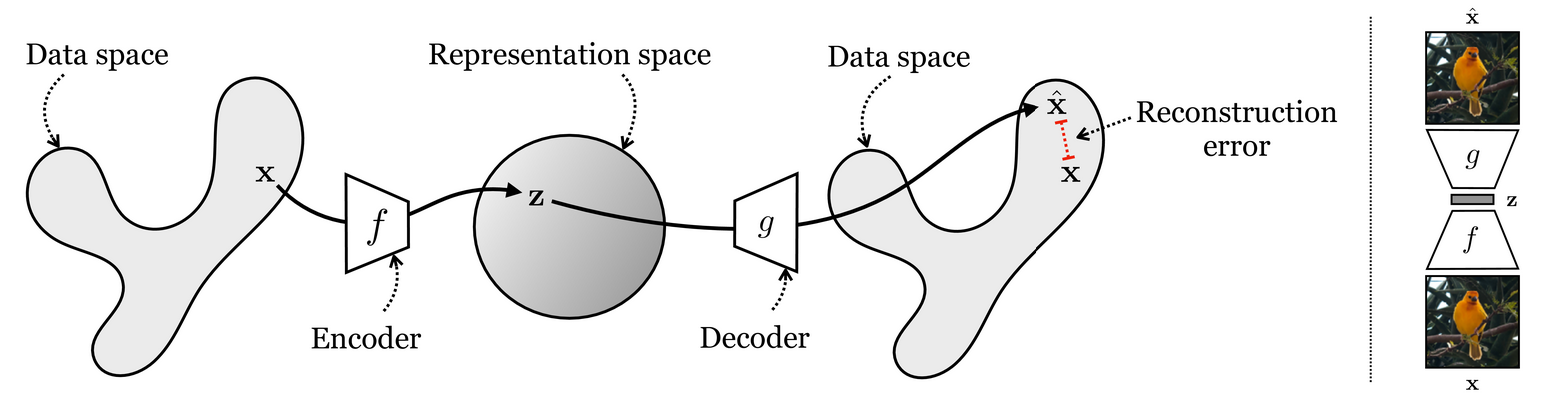
\includegraphics[width=\columnwidth]{autoencoder.png}}
\caption{A digram of image reconstruction using Autoencoders, taken from \cite{foundationsCVbook}. The encoder learns to compress the image into a smaller feature vector, while the decoder learns to to reconstruct the original image using this representation. The goal is to reconstruct the original image as closely as possible.}\label{fig:autoencoder}
% \vskip 0.5in
\end{figure} 

Image understanding is useful for many machine learning applications such as classification or generation. Raw image data however is high-dimensional and contains sparse signal, which can lead to poor convergence when training naively. In this paper we study a class of neural networks called Autoencoders \cite{foundationsCVbook}, which are designed to compress images through an encoder and reconstruct the original image through a decoder \ref{fig:autoencoder}. The main goal is to get the encoder to learn useful representations of the original image that preserve most of the signal in a lower dimensional space. We further investigate the effectiveness of contrastive learning \cite{foundationsCVbook} with the goal of training the encoder to produce representations that are invariant to fixed transformations, such as the shape of objects or their colors. This project type aims to recreate both the autoencoder and contrastive learning experiments contained in Chapter 30 of the Computer Vision textbook \cite{foundationsCVbook}.

\section{Motivation}

Consider a dataset of points $\mathbf{x} \in \mathbb{R}^N$. 

\textbf{For Image Reconstruction}, given datapoints $\mathbf{x} \in \mathbb{R}^M$ draw from some distribution, we are given encoder $f: \mathbb{R}^N \to \mathbb{R}^M$, decoder $g : \mathbb{R}^M \to \mathbb{R}^N$, where $N << M$. Our goal is to then learn $f^*, g^*$ such that 

\[ f^*, g^* = \underset{f, g}{\text{argmax}} \mathbb{E}_{\textbf{x}} \norm{ g(f(\textbf{x})) - \textbf{x}}^2_2 \]

from $\cite{foundationsCVbook}$. Initutively, we should expect our encoder $f(\textbf{x}) = \textbf{z}$ to learn a useful representation $\textbf{z} \in \mathbb{R}^M$ that retains most of the information in the original image. We then want $g(\textbf{z}) = \hat{ \textbf{x} }$ to learn how how to use this representation to reconstruct the original image. We can then use networks we can then use it for data compression and interpolation, or to study the feature learning capabilites of neural nets directly.

\begin{wrapfigure}{r}{0.5\textwidth}
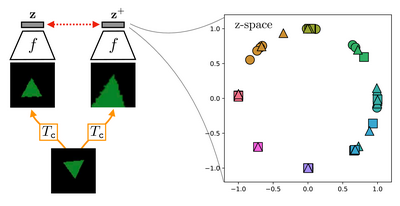
\includegraphics[scale=0.70]{contrastive_learning.png}
\caption{A digram of contrastive learning taken from \cite{foundationsCVbook}. Here the cropping transformation helps the encoder to produce embeddings that are close to each other if they share the same color.}\label{fig:contrast_learn}
% \end{center}
% \vskip 0.5in
\end{wrapfigure}


\textbf{For Contrastive Learning}, given some datapoint $\mathbf{x} \in \mathbb{R}^d$, similar (positive) datapoints $\mathbf{x}^+$, and disimilar (negative) datapoints $\mathbf{x}^-$, we aim to minimize $D(\textbf{x}, \textbf{x}^+)$ and maximize $D(\textbf{x}, \textbf{x}^-)$, where $D$ is some distance function \ref{fig:contrast_learn}. In practice, we may take $\textbf{x}^+ = T(\textbf{x})$, where $T$ is a chosen transformation applied to our dataset (e.g. cropping) to preserve certain features, while $\textbf{x}^-$ may be randomly sampled from our dataset \cite{foundationsCVbook}. Compared to simply taking the encoder from image reconstruction, contrastive learning helps our encoder learn to produce embeddings that are clustered by common features determined our transformation. This is useful, for instance, if we want our encoder to cluster images based on specific properties like shape or color - using image construction only does not guarentee that our encoder will be invariant to transformation. 

\section{Approach}

\subsection{Image Reconstruction}

\subsubsection{Baseline}
We first experimented with a fully connected multi-layer-perceptron as our autoencoder baseline. We noticed several issues when trying to train it however, namely poor convergence and that the images produced were unsmooth. Due to the extremely poor performance of this baseline, we omit the results from this final report.

\subsubsection{Advanced}

For image reconstruction, we next tried using a convolution neural network for both the encoder and decoder. We chose this approach due to the fact that CNNs are more naturally suited to image tasks, due to the sparsity of signal on image data specifically (as discussed in class). Our encoder first downsamples the image data into a representation of $M$ size using convolution, while the decoder upsamples the representation through multiple transposed convolutional layers. We choose our loss to be MSE between the original and reconstructed data point.

\subsection{Contrastive Learning}

\subsubsection{Baseline}
After building a convolutional encoder from our Image Reconstruction experiments, we then experimented with training our encoder using InfoNCE loss for a given image transformation. However, we found that using InfoNCE was very inconsistent for our dataset, and sometimes lead model training to fail to converge. 

\subsubsection{Advanced}

We then pivoted toward using triplet loss instead, which defined as 

\[ \mathcal{L} (\textbf{x}, \textbf{x}^+, \textbf{x}^-) = \max(D(f(\textbf{x}), f(\textbf{x}^+)) - D(f(\textbf{x}), f(\textbf{x}^-)) + m, 0) \]

where $f$ is our autoencoder, $D$ is our distance function, and $m$ is our margin \cite{foundationsCVbook}. We use the $\ell2$ norm is our $D$ function in our experiments.

We find using triplet loss was much faster and more consistent. We believe that the better performance of triplet loss is due to the fact that InfoNCE uses dot product to compute distances between vectors, which becomes problematic when a lot of the image has no values (e.g empty regions).

\subsection{Libraries and Resources}

We primarily use the torch and torchvision libraries to import our dataloader and dataset objects, as well as transforms, model components, etc. We also use the pillow library to work with images, and matplotlib for visualizations.

As our models are relatively small, we are able to successfully train our model on our local devices without much issue.

\section{Experiments}

\subsection{Data}
To evaluate the performance of our autoencoder, we first generate a dataset of 50,000 128x128 images of single, simple shapes (e.g. triangles, circles, squares) of different colors, sizes, and orientation, and save them using the Pillow library. 

In our models, we set $M = 128$ as the dimension for our encoder output embedding. We also use the the Adam optimizer with learning rate $0.001$, and train for $100$ epochs with a batch size of $32$ for both experiments. 

\subsection{Metric} We also use the training loss directly to measure the performance our of models, and qualitative analysis to estimate the final results. For Image reconstruction, we simply compare the reconstructed image with the original image. We achieved a validation loss of 0.00027 on a validation set of 5,000 images, where RGB values are normalized between 0 and 1. For contrastive learning, for any output embedding we find the nearest 5 embeddings within the dataset. For contrastive learning we also experiment with two types of transformations: cropping and recoloring the shapes within an image. The main aim of these transformations is to learn embeddings that are invariant to color and shape, respectively. As such, we primarily do qualitative analysis based on human judgement.

\subsection{Results}

\subsubsection{Image Reconstruction}

\begin{wrapfigure}{r}{0.5\textwidth}
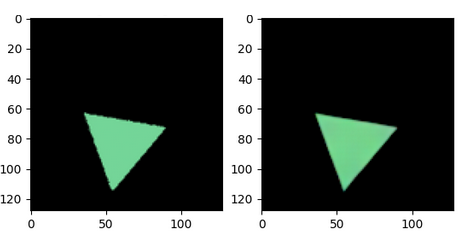
\includegraphics[scale=0.5]{autoencoder_results.png}
\caption{Example output from our autoencoder. The reconstructed image strongly resembles the input image, minus some smoothed edges}\label{fig:autoencoder_res} 
% \end{center}
% \vskip 0.5in
\end{wrapfigure}

In our autoencoder, we set our encoder to use 5 layers of convolution + nonlinearity, and our decoder to use 4 layers of tranposed convolution blocks (see codebase for more details). We use the MSE loss in this scenario.

For image reconstruction, we are able to achieve a reconstruction loss of $\leq 0.002$, despite compressing the image to a much smaller embedding. We are also able to visually inspect the output images and see that they strongly resemble the original iamge, as in \ref{fig:autoencoder_res}. We also interpolate the learning process in the autoencoder and see that it is able to smoothly learn features from different images; we omit a diagram in this report due to the inability to import GIF files into pdf, but include it in our slides.

\subsubsection{Contrastive Learning}

For contrastive learning, we use 7 layers of convolutions in our encoder and remove the last MLP. We also use the triplet loss of temperature of $0.5$ and a margin of $0.3$ after some hyperparameter testing; we find our baseline approach using InfoNCE to be too weak to gather tangible results. For each experiment, we form positive samples $\textbf{x}^+ = T(\textbf{x})$ for some fixed transformation $T$, and find negative samples by sampling iid from the same batch.

\begin{figure}[ht]
% \centering
\centerline{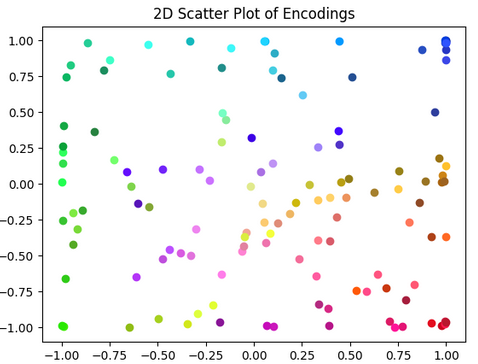
\includegraphics[scale=0.7]{contrastive_scatter.png}}
\caption{A scatterplot of output embeddings of the encoder, where $T$ is a random crop. Each dot represents the actual color of the shape in each image. Using the cropping transformation, our encoder learns to cluster images of similar colors into distinct regions.}\label{fig:contrastive_scatter}
% \vskip 0.5in
% \vskip 0.5in
\end{figure} 

  

We first experiment with contrastive learning using cropping transformation. As noted in \cite{foundationsCVbook}, this simple transformation is sufficent to enable the encoder to learn to produce color-invariant embeddings. We verify the findings in the book and plot our results as in \ref{fig:contrastive_scatter}, and note that our encoder naturally seperates images of distinct colors into distinct regions.

We note however that the delineation is not necessarily seperable for certain colors, nor do colors cluster smoothly with respect to each other. For instance, we see yellows clustered together, but that some yellows are closer to blue than green despite yellow being a direct component in green. We hypothesize this is due to the fact that the positive samples are only chosen up to cropping of the same image, and so the model does not necessarily need to learn to cluster different colors relative to each other. We leave learning such representations as an extension for future work. 


\begin{figure}[ht]
% \centering
\centerline{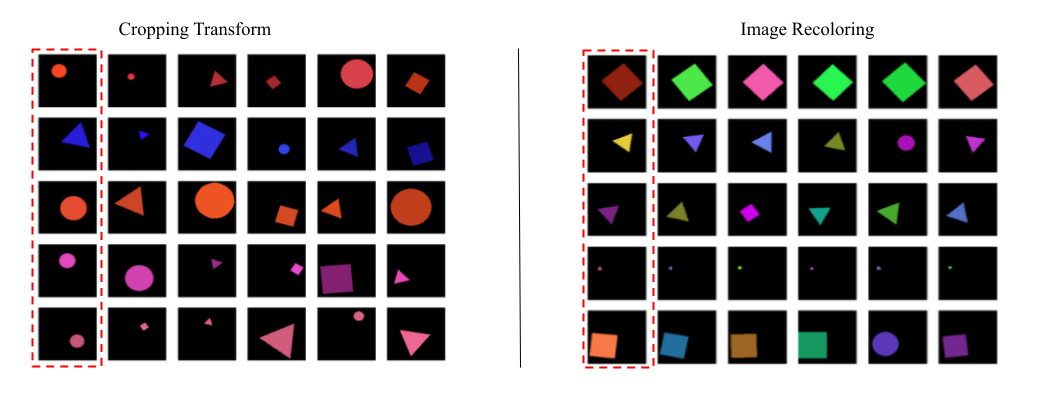
\includegraphics[scale=0.45]{contrast_learning_transforms.png}}
\caption{Side by side comparison of the $k$-nearest neighbors (row) to an input image (dotted boxes) in the output representation space. As seen on the left, under cropping the encoder learns to cluster images of similar colors together, while under image recoloring the clustering is based on shape instead. }\label{fig:contrastive_transforms}
% \vskip 0.5in
% \vskip 0.5in
\end{figure}   

We also experiment with recoloring the shape in the original image to a different color as our transformation, and find that our encoder is able to learn to seperate images invariant of color and focus more on the image shape instead. As an inadvertent consequence however, we see that the encoder is also sensitive to orientation. See \ref{fig:contrastive_transforms} for reference.

\section{Conclusion}

\subsection{Insights}
As a result of our experiments, we are able to successfully reproduce the experiments in \cite{foundationsCVbook}. Insights gained along this process include more direct experience in working with machine learning libraries, as well as the importance of introducing the right inductive biases within our model, whether that be in choices of archiecture or training objective. Through our experiments in autoencoders, we are able to demonstrate the effectiveness of neural data compression for efficent learning. Furthermore, through our experiments in contrastive learning, we are able to demonstrate that simple modifications in our loss is sufficent for our encoder to learn property-invariant features. We also gained insight into building effective transforms for enabling robust feature representations.

\subsection{Workload}
Our workload included generating the dataset, creating the autoencoder and contrastive learning encoder, iterative experimentation, generating visualizations, extending the experiments, and creating documentation and reports. All team members contributed evenly to most parts, however Shashank contributed moreso to the dataset creation and autoencoder, Kevin worked on both the autoencoder and contrastive learning, and Michael worked on the autoencoder and contrastive learning as well.


\subsection{Key Challenges}
Key challenges faced during this project include issues with trying to train the baseline MLP, which we found to be too weak despite multiple iterations. We also spent a lot of time trying to train the contrastive learning encoder using InfoNCE, but were unable to get consistent model convergence. As this varied depending on the random inialization and choice of batches, we believe that InfoNCE happened to provide very weak signal for gradient descent, and so was unable to train effectively. We also scrapped building our own autograd engine due to time limitations and the fact we believed it was not as valuable of a learning experience for machine learning directly.

\subsection{Final Remarks}
We therefore found this project to be highly applicable into applying machine learning in the computer vision domain. We find the learning experience to be worthwhile and insightful, and identify numerous directions for continous improvement and learning. 

% \section*{References}

\bibliography{sources}

% References follow the acknowledgments in the camera-ready paper. Use unnumbered first-level heading for
% the references. Any choice of citation style is acceptable as long as you are
% consistent. It is permissible to reduce the font size to \verb+small+ (9 point)
% when listing the references.
% Note that the Reference section does not count towards the page limit.

%%%%%%%%%%%%%%%%%%%%%%%%%%%%%%%%%%%%%%%%%%%%%%%%%%%%%%%%%%%%

% \appendix

% \section{Technical Appendices and Supplementary Material}
% Technical appendices with additional results, figures, graphs and proofs may be submitted with the paper submission before the full submission deadline (see above), or as a separate PDF in the ZIP file below before the supplementary material deadline. There is no page limit for the technical appendices.

%%%%%%%%%%%%%%%%%%%%%%%%%%%%%%%%%%%%%%%%%%%%%%%%%%%%%%%%%%%%

\end{document}